

% %%%%%%%%%%%%%%%%%%%%%%%%%%%%%%%%%%%%%%%%%%%%%%%%%%%%%%%%%%%%%%%%%%%%%%%%%%%%%%%%%





\chapter{Lab: Design and analysis of LNAs}

\section{Introduction}

\section{Creation of your Library and LNA cell}


\section{First simulation of the circuit}
\begin{pexbox}{}
   \noindent \textbf{Capture the windows containing your design selections (Schematic, Variables section of the ADE window). Include them in your report.}
\end{pexbox}

\noindent Although my pre-lab calculations were pretty close to the ones provided by the professor, I ended up using his numbers, as we were told they would let us obtain very good results without tunning much the circuit.
\begin{figure} [H] \centering
   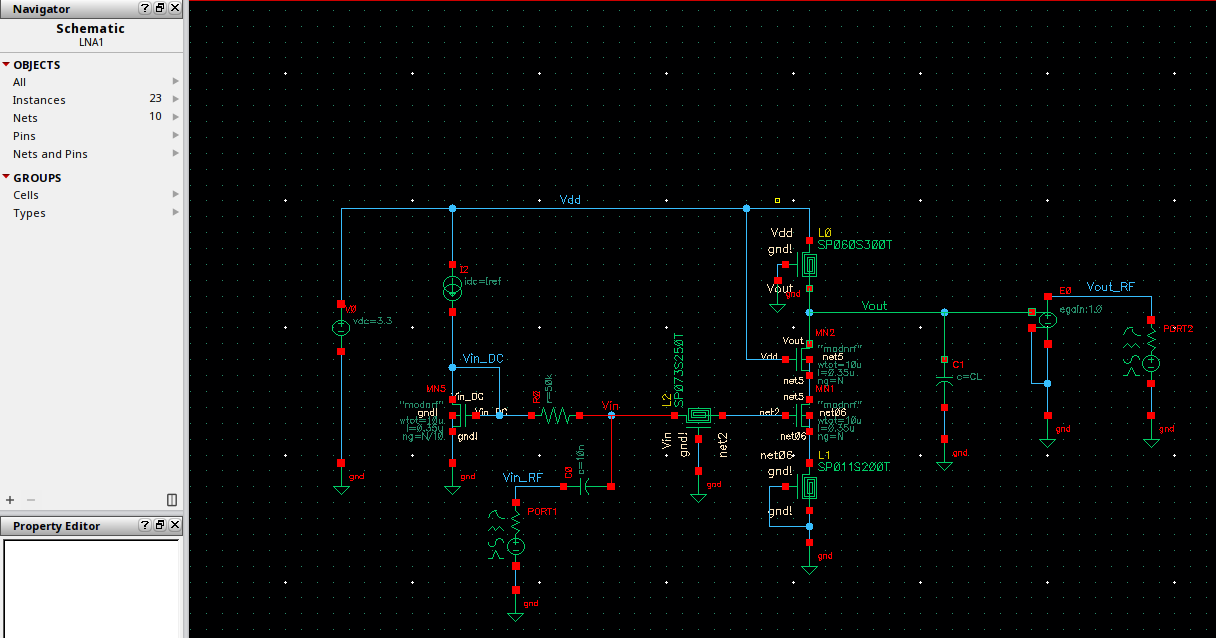
\includegraphics[scale=0.45]{schematic-3-1.png}
   \caption{Schematic}
\end{figure}

\begin{figure} [H] \centering
   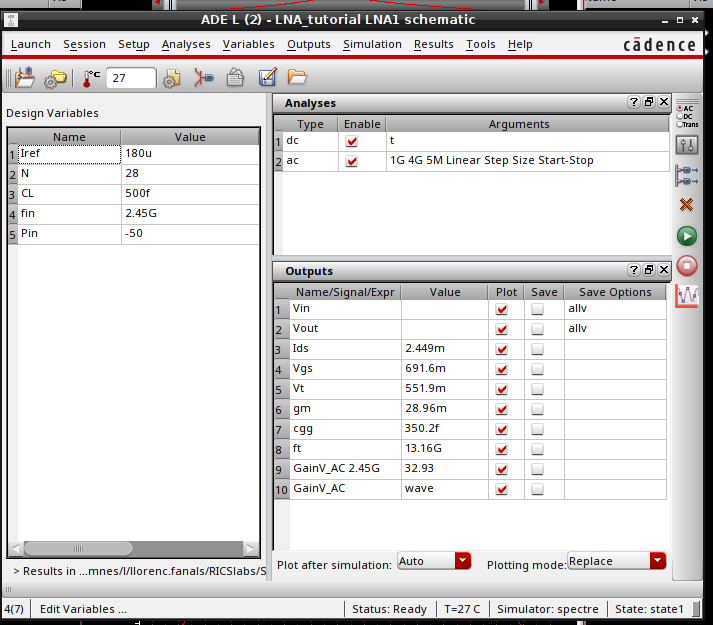
\includegraphics[scale=0.5]{ade-3-1.png}
   \caption{ADE window}
\end{figure}




\begin{pexbox}{}
   \noindent \textbf{Create a small table comparing the OP parameter values against the values expected according to your prelab calculations. Include them in your report.}
\end{pexbox}

   \noindent As commented, I use the numbers provided by the professor, and for $V_{TH}$ I take the value that appears on the technology data table.
   \begin{table}[H] \centering
      \begin{tabular}{ |l|r|r| } \hline
          Characteristic & Theoretical value & Simulation value \\ \hline \hline
          $I_{DC}$ & $2.5$ mA & $2.449$ mA \\ \hline
          $V_{GS}$ & $0.6822$ V & $0.6961$ V \\ \hline  
          $V_{TH}$ & $0.5$ V & $0.5519$ V \\ \hline
          $g_m$ & $24.7$ mA/V & $28.96$ mA/V \\ \hline
          $C_{GG}$ & $350$ fF & $350.2$ fF \\ \hline
          $f_T$  & $11.2$ GHz & $13.16$ GHz \\ \hline
      \end{tabular}
      \caption{Parameter comparison}
   \end{table}
\noindent The results are smilar in most cases. The transconductance $g_m$ is higher for the simulation, thus leading to a higher $f_T$ value, too. This is something positive, we can get a higher gain for the same power consumption.

\begin{pexbox}{}
   \noindent \textbf{Capture the results of the AC analysis, including markers measuring the ressonance frequency and voltage gain.}
\end{pexbox}


\begin{figure} [H] \centering
   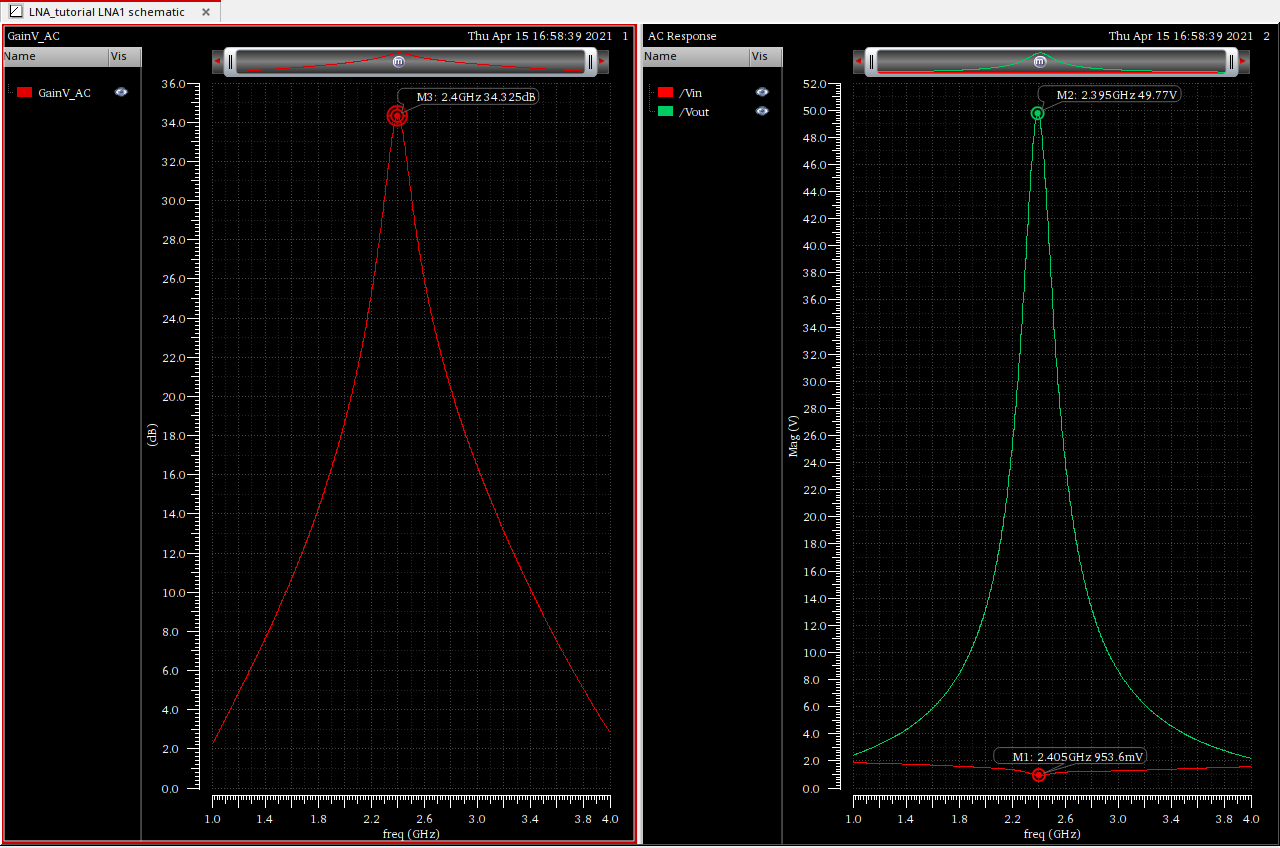
\includegraphics[scale=0.45]{plots-3-2.png}
   \caption{Gain and voltage plots}
\end{figure}

% \noindent From the plots, the ressonant frequency is at $2.4$ GHz. The gain is higher than $30$ dB, which was the gain for which the design was made. This is thanks to the unexpected increase in $g_m$ that appears in the simulation.
\begin{equation}
   |A_v| = 34.325 \text{ dB} \ .
\end{equation}

\begin{pexbox}{}
   \noindent \textbf{Can you extract some information on the input matching, from the plots obtained?}
\end{pexbox}

\noindent I extract that input matching must be very good because the obtained gain is higher than $A_v = 30$ dB, which was the gain we pursued in the pre-lab. Part of this comes from the fact that the $g_m$ obtained is greater than the theoretical one, but in spite of this we wouldn't obtain this large gain if it was not for very good input matching, which is evaluated in the following section.




\section{Evaluating Gains and Input Matching}
\begin{pexbox}{}
   \noindent \textbf{Capture the plot of the S11 parameter, including markers to measure the ressonance frequency of S11 and its value at $f_0 = 2.45$ GHz.}
\end{pexbox}

\begin{figure} [H] \centering
   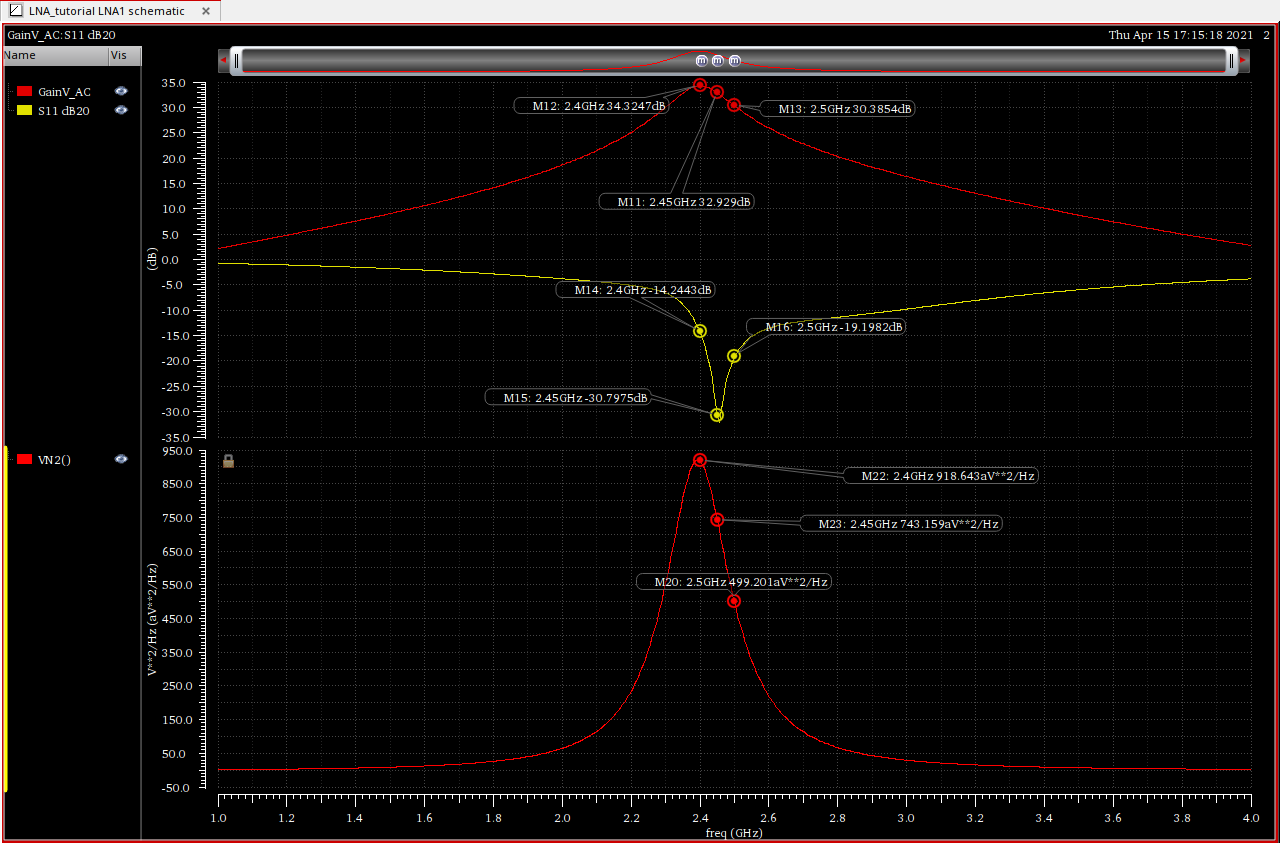
\includegraphics[scale=0.45]{4-2-s11-plots.png}
   \caption{Gain and S11 plots}
\end{figure}

\noindent While $f=2.45$ is not the frequency for which the gain is at its maximum, it is the frequency for which the input matching is best.
\begin{equation}
   S_{11}|_{2.45 \text{ GHz}} = -30.7975 \text{ dB} \ .
\end{equation}
\noindent This fulfils the $S_{11}$ specification without a problem, which consisted on $S_{11} < -10$ dB. 

\noindent Around $f_0$, the central frequency, the S11 parameter shows very small values. This means that the ratio between the reflected wave and the incident wave is very low (if perfectly isolated, as is the case thanks to the buffer, S11 is just this relation). This is something desired because it means that almost no power will be lost in the input stage, so it can be concluded impedance matching is very good. 

\noindent Recall,
\begin{equation}
   \begin{pmatrix}
      V_1^- \\
      V_2^+
   \end{pmatrix} = \begin{pmatrix}
      S_{11} & S_{12} \\
      S_{21} & S_{22} 
   \end{pmatrix} \begin{pmatrix}
      V_1^+ \\
      V_2^-
   \end{pmatrix} \ .
\end{equation}



\begin{pexbox}{}
   \noindent \textbf{Capture the plots of the impedance, including markers at $f_0 = 2.45$ GHz.}
\end{pexbox}
   
   \noindent Now, the input impedance is obtained, both the real and imaginary parts. Recall that, ideally, the imaginary impedance should be $0$ at $f_0$ and the real impedance should be $50 \ \Omega$. The closer to these values, the better.
\begin{figure} [H] \centering
   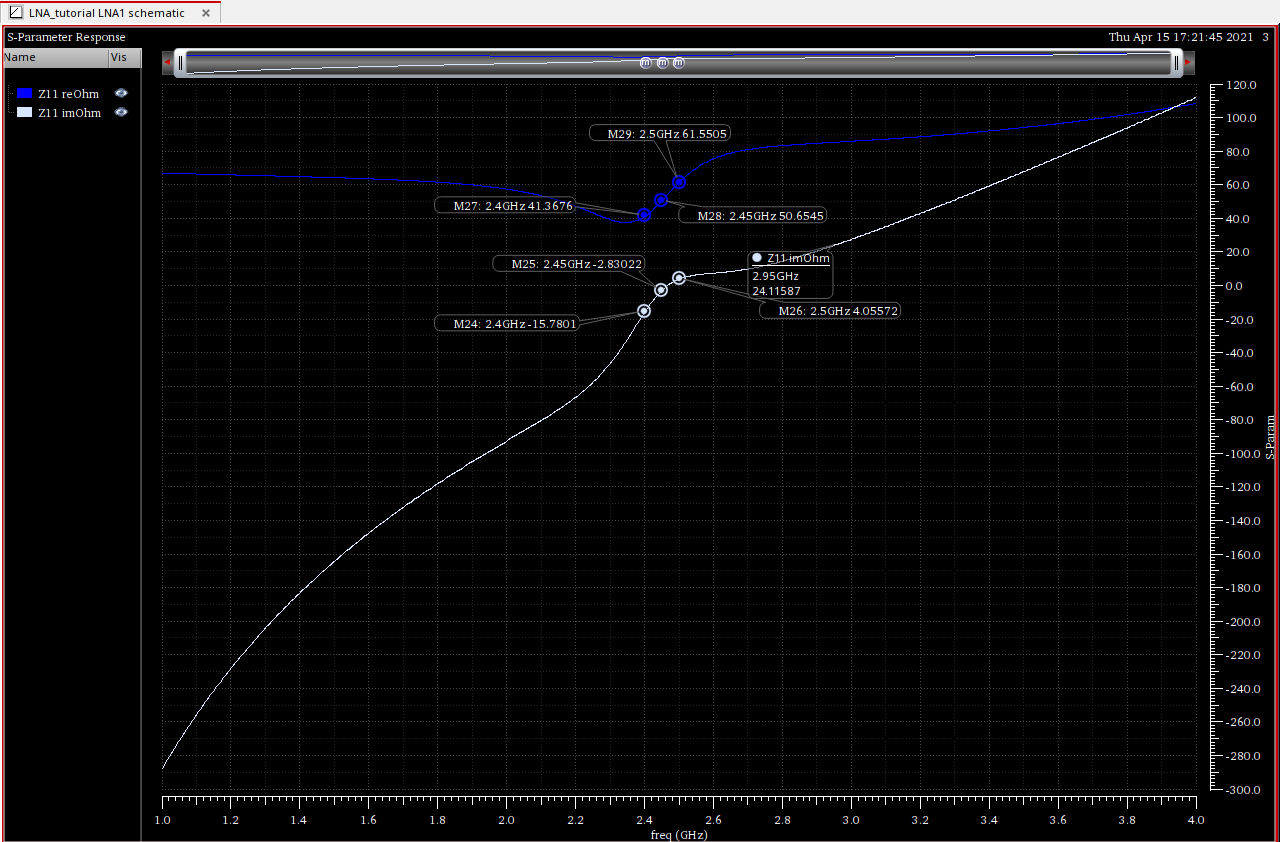
\includegraphics[scale=0.45]{4-2-z11-imag-real.png}
   \caption{Z11 plots}
\end{figure}

\noindent Notice the real impedance at $2.45$ GHz is very close to $50 \ \Omega$, and that the imaginary part is $-2.83022 j \ \Omega$. So, the source impedance is very close to being matched by the amplifier input impedance. This explains the good $S_{11}$ parameter.


\begin{pexbox}{}
   \noindent \textbf{Compare the values obtained, to the targeted ones.}
\end{pexbox}

   \noindent Ideally, the amplifier input impedance should be equal to the voltage source output impedance: a real $50 \ \Omega$. Matching is not perfect but very close to it. By using the professor's numbers, I avoid having to tune the design. I already get a very low S11 parameter and a gain above $30$ dB.


\noindent Also, I've obtained the Smith chart:
\begin{figure} [H] \centering
   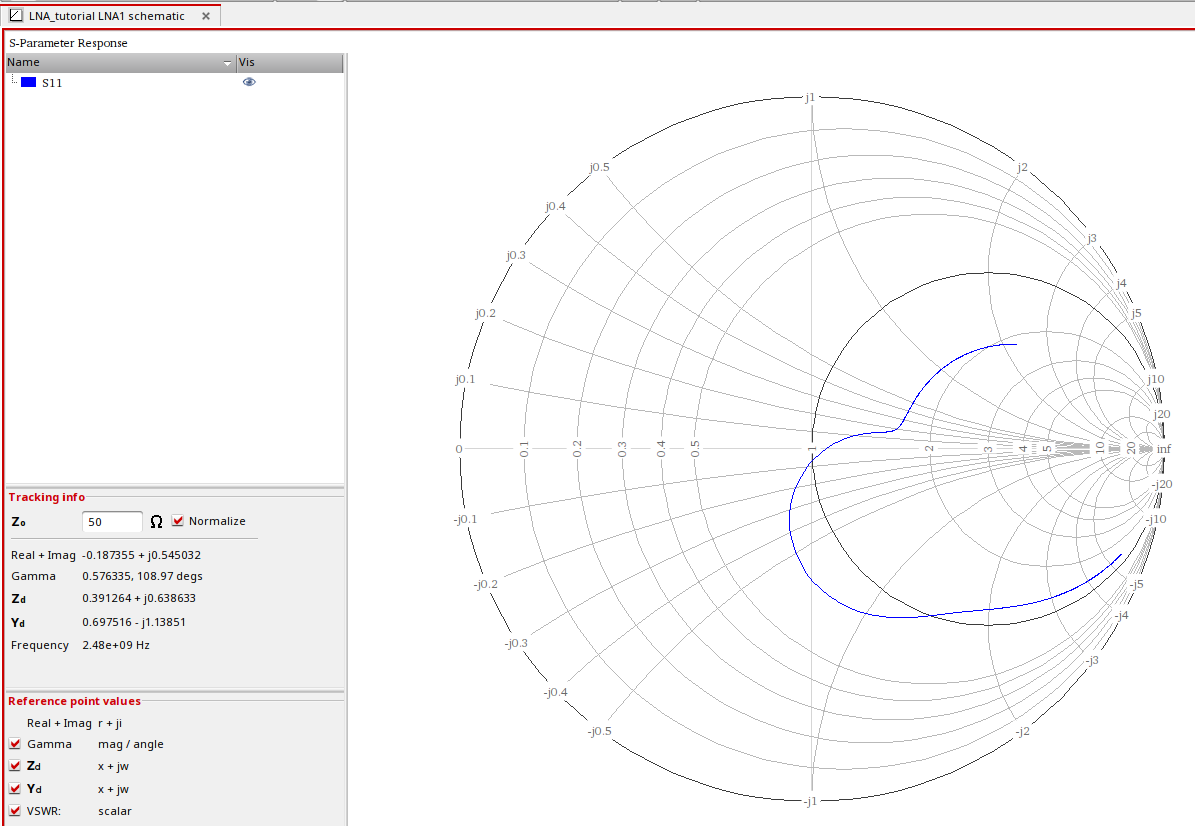
\includegraphics[scale=0.45]{smith.png}
   \caption{Smith chart}
\end{figure}

\noindent Notice the plot, in blue, crosses the unit circle around $-0.05 j$. Considering it is normalized to $50 \ \Omega$, as commented on the laboratory document and as appears in the plot itself, this would lead to $\approx -2.5j$, which is very close to the actual obtained value, $-2.83022 j \ \Omega$. As the cross is not in the center of the plot, matching is not perfect, but it's quite close to it.



\begin{pexbox}{}
   \noindent \textbf{Capture the plots, including markers at $f_0 = 2.45$ GHz.}
\end{pexbox}

   \noindent Now, we are interested in the gain from input to output. Notice from the previous equation that $S_{21}$ relates the $V_2^+$ to $V_1^+$. $V_2^-$ in theory also affects, but in principle $S_{22}$ is very low. The transducer power gain, $G_T$, and the operating power gain $G_P$, are
   \begin{equation}
      \begin{split}
         G_T &= 10 \log \left( \frac{P_{OUT}}{P_A}\right) = 10 \log(|S_{21}|^2) \\
         G_P &= 10 \log \left(\frac{P_{OUT}}{P_{IN}}\right) = G_V + 10 \log \left( \frac{R_{in}}{R_{L}}\right) = 10 \log \left( \frac{|S_{21}|^2}{1 - |S_{11}|^2} \right)
      \end{split} \ .
   \end{equation}
   \noindent If $|S_{11}|$ is very low, which as seen previously is true, and can approximate $S_{11} \approx 0$, then $G_T = G_P$, i.e., the trasducer power gain is equal to the operating power gain. For frequencies far from the ressonant frequency, high differences can be expected between $G_T$ and $G_P$, because $S_{11}$ is not longer approximately $0$, which means that input matching is no longer close to perfection. Next, the $S_{21}$, $G_T$ and $G_P$ plots are shown.

\begin{figure} [H] \centering
   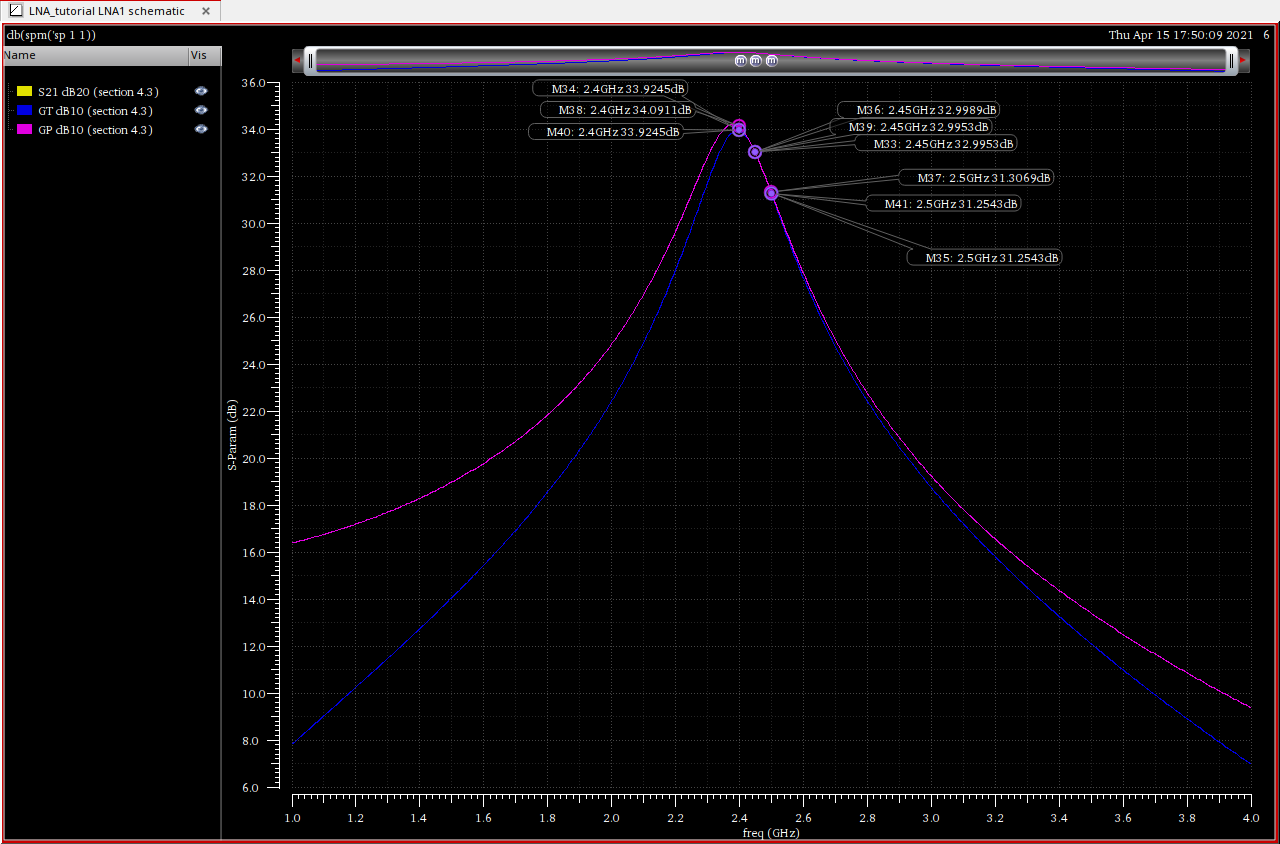
\includegraphics[scale=0.45]{4-3-gs.png}
   \caption{GT, GP, S21 plots}
\end{figure}

\noindent The $S_{21}$ plot is overlapped with the $G_T$ plot. It makes sense according to the definition I've just given. When there is not a good input matching (for frequencies far from the central one), the input power is lower than the one provided by the voltage source and thus $G_P > G_T$, because there's no perfect impedance matching, and thus $P_{IN} < P_{A}$. The $G_P$ resembles a lot the gain plot I showed before. Anyways, the differences between the three plots are minimal in the expected frequencies.


\begin{pexbox}{}
   \noindent \textbf{Are the results obtained consistent with the theoretical expectations?}
\end{pexbox}

\noindent Yes, when there's good input matching (around the central frequency), the gain is over $30$ dB, as desired. And when there's not good input matching, which is something that happens for frequencies far from the central one, the gain is much lower. Also, we know $G_P$ is more "optimistic" than $G_T$; the port component provides the specified power to the amplifier, at the cost that far from the central frequency $P_A$ must be considerably higher than $P_{IN}$, i.e., not all the available power at the source arrives at the input of the amplifier.




   \noindent Now, I've changed the PORT2 impedance to $500 \ \Omega$. Keep in mind the original schematic: the output port, PORT2, was connected to a 4-port component that copied the voltage at its two input ports to its two output ports, i.e., a simple buffer. So, the gain shown by the amplifier itself, defined as the output voltage divided by the input voltage, should not change in spite of increasing the output impedance. 


\begin{pexbox}{}
   \noindent \textbf{Measure the four gain values at $f_0 = 2.45$ GHz.}
\end{pexbox}

\begin{figure} [H] \centering
   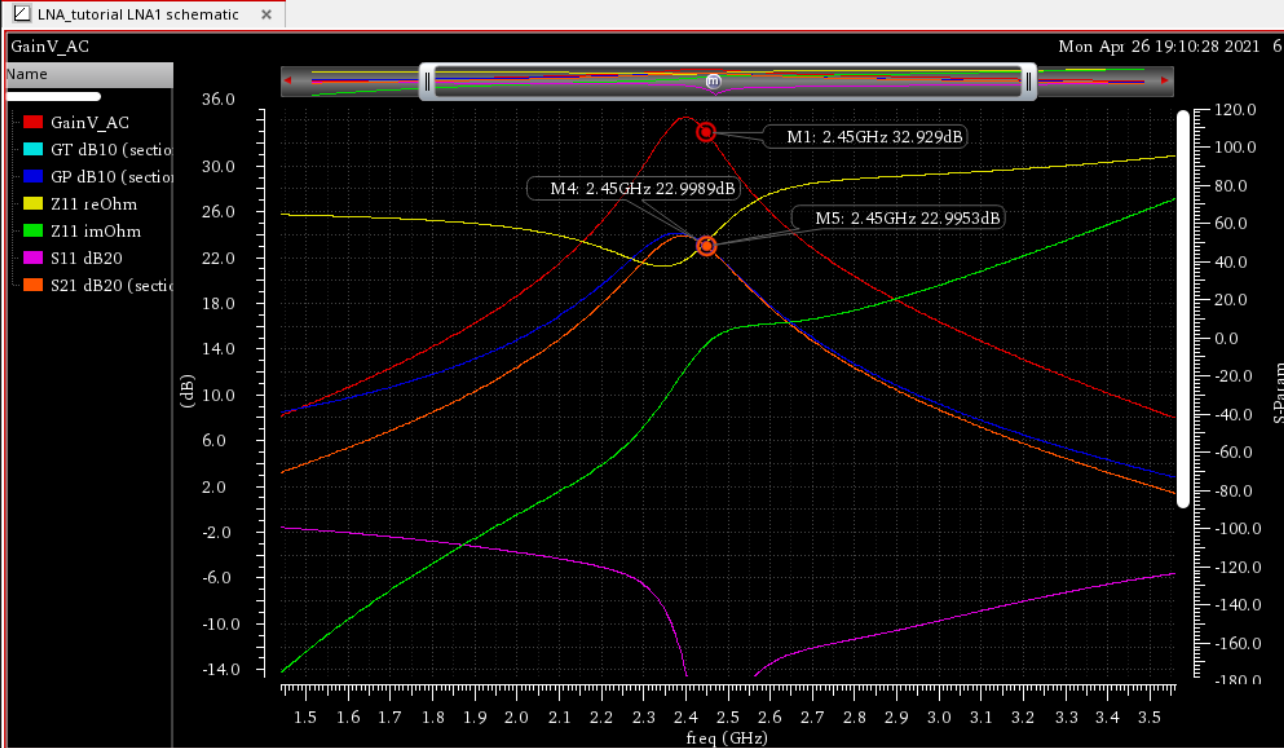
\includegraphics[scale=0.45]{4-3-500ohm.png}
   \caption{Plots}
\end{figure}

\noindent Again, the $S_{21}$ plot is overlapped to the $G_T$.

\begin{pexbox}{}
   \noindent \textbf{Are the results obtained consistent with the theoretical expectations?}
\end{pexbox}

\noindent By increasing the output impedance by a $10$ factor, the $10 \log \left( \frac{R_{in}}{R_{L}}\right)$ term decreases by $10$ dB. This happens to $G_P$, clearly from the equation, and also to $|S_{21}|$ and thus $G_T$. This is the reason for the $10$ dB shift.




\begin{pexbox}{}

   \noindent Next, I've added a $100 \ \Omega$ series resistance with $L_G$.

   \noindent \textbf{Capture the plots of the four gains, and the S11 parameter, including markers at $f_0 = 2.45$ GHz.}
\end{pexbox}


\begin{figure} [H] \centering
   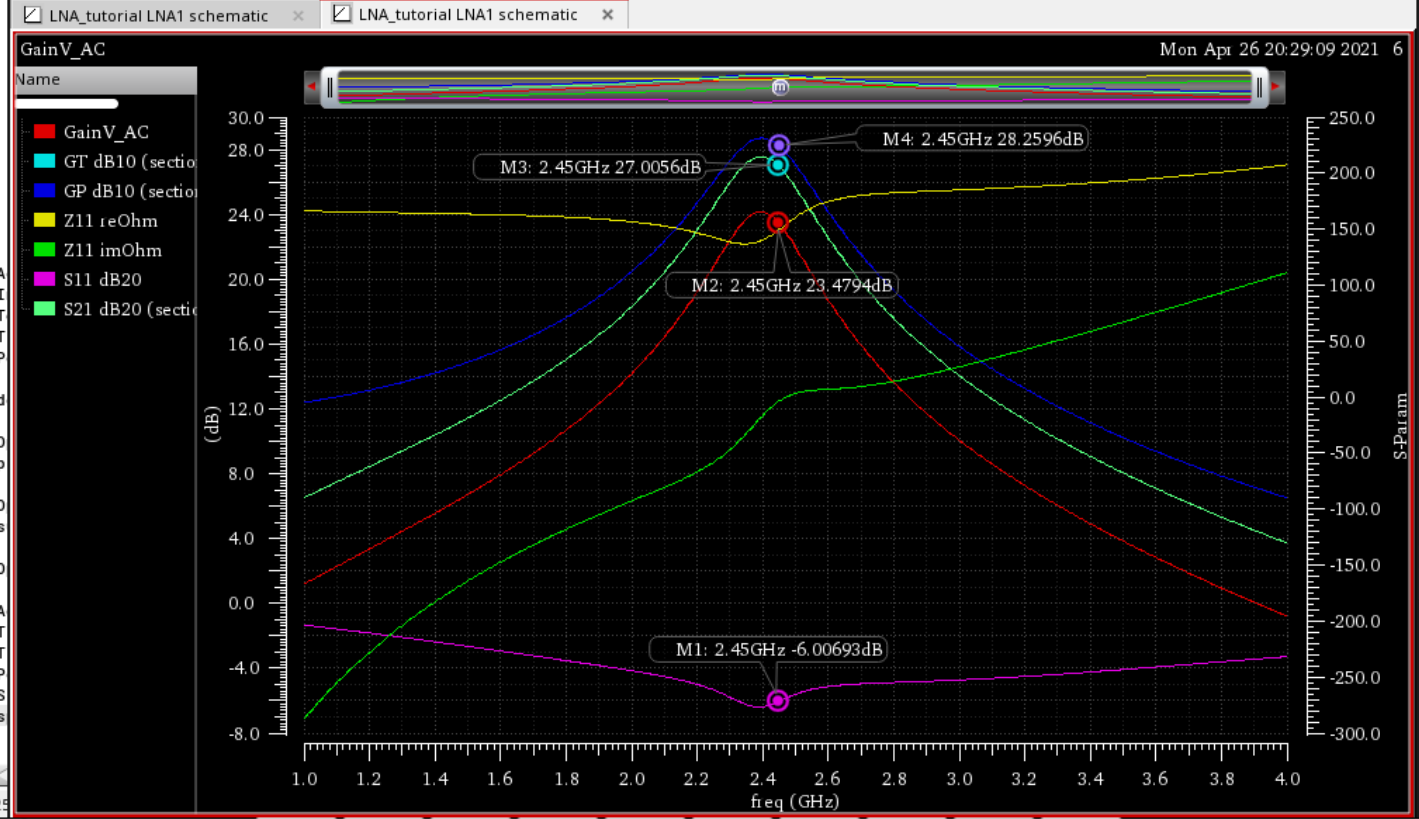
\includegraphics[scale=0.4]{4-3-100ohm.png}
   \caption{Plots}
\end{figure}

\noindent Again, the $S_{21}$ plot is overlapped to the $G_T$.

\begin{pexbox}{}
   \noindent \textbf{Are the results obtained consistent with the theoretical expectations?}
\end{pexbox}
   
\noindent Now, there's no input matching at the central frequency. Recall we've verified our circuit was quite good at showing a real $50 \ \Omega$ input impedance at $f_0$. Now, by adding a resistance of $100 \ \Omega$ in series with the gate inductance, clearly $S_{11}$ won't be as low as before, meaning there will be a partial reflection at the input and thus the output power will be lower. At the same time, this will mean the output gain will be lower.

\noindent Before, it was shown that we had $S_{11} = -30.7975$ dB. Now, this is just $-6$ dB. For the $G_V$ gain, I notice the linear factor between the previous gain and the current one is very close to $3$. It makes sense if one considers that only $1/3$ of the voltage at the input node reaches the circuit we had before, i.e., $2/3$ of voltage fall at the $100 \ \Omega$ resistance. 

\noindent $G_T$ and $G_P$ also result affected by this. From previous expressions, it can be seen that $G_T - 10 \log(1 - |S_{11}|^2) = G_P$. The plotted $S_{11}^2 = -6 \text{ dB} = 0.2512$, so $10 \log(1- |S-{11}|^2) = 0.7488 = -1.256$ dB, which is almost exactly the difference $G_P - G_T$. The $G_P$ gain has also been reduced $-6$ dB from its original value, because of bad input matching.  
% revisar 4port components i justficiar els GT i GP





\section{Evaluating Isolation and Stability}
\begin{pexbox}{}
   \noindent \textbf{Capture the plot evaluating the reverse isolation, including marker at $f_0 = 2.45$ GHz.}
\end{pexbox}

\begin{figure} [H] \centering
   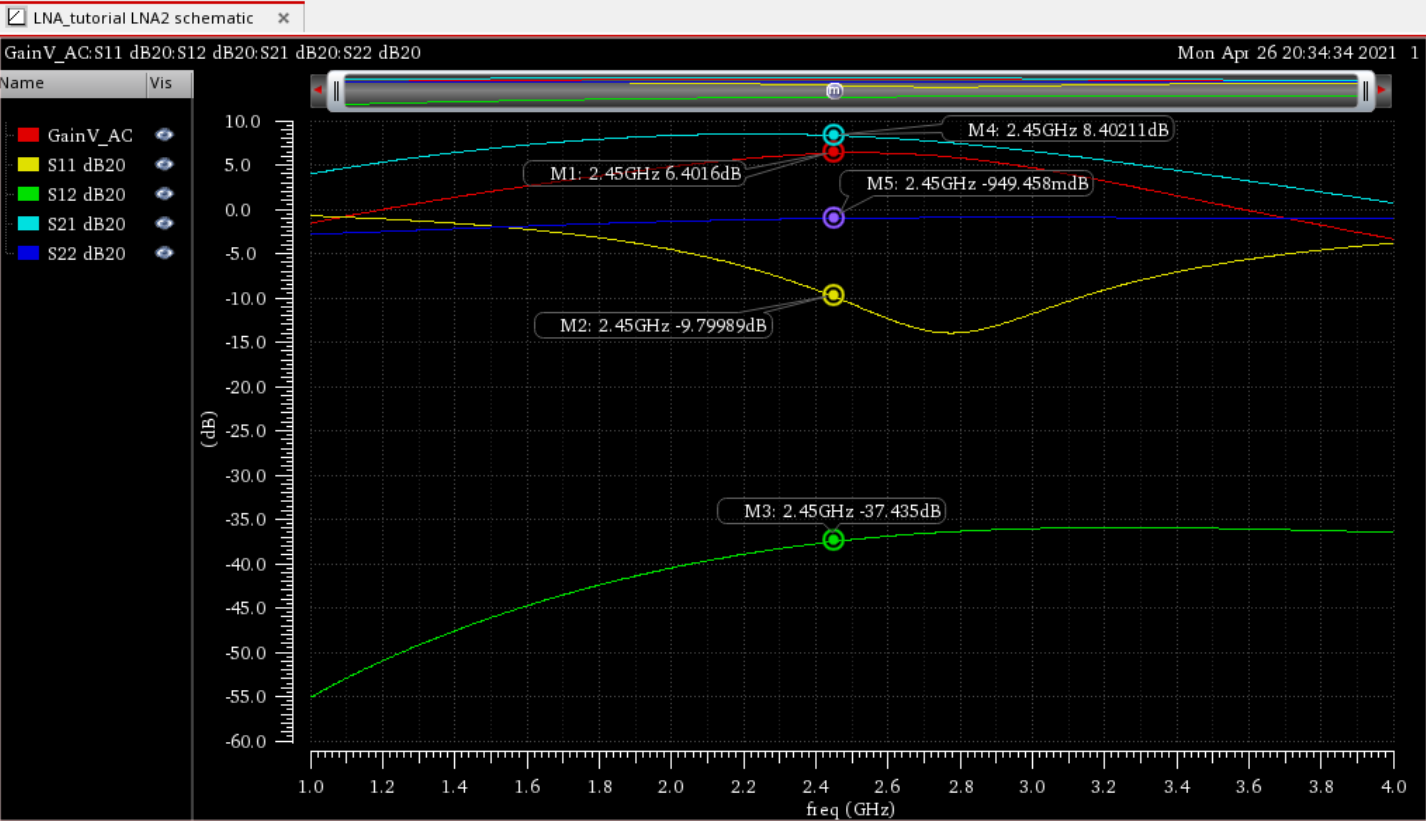
\includegraphics[scale=0.4]{5-2.png}
   \caption{S parameters and gain plots}
\end{figure}


\begin{pexbox}{}
   \noindent \textbf{Does the reverse isolation have a good value?}
\end{pexbox}

   \noindent Although it could always be lower, in a linear scale $S_{12} \approx 0.014$, so the contribution to $V_{1}^-$ by the output is almost "only" $1$\% of the output voltage. However, keep in mind the output voltage is amplificated by around $30$ dB (in fact, from simulations it was around $33$ dB). So, the input voltage is amplified by the amplifier, and then part of this amplified signal is fedback to the input. The fedback signal is $\approx -4$ dB with respect to the input signal.
   
   \noindent We already have the cascode transistor that helps quite a lot in isolating the output and the input (mainly the Miller capacitance that would appear with a single transistor does not longer appear with the cascode). So, I don't think there's much more to do to improve the $S_{12}$ parameter. Keep in mind the comment made in the document lab, it suggests that this output loading would not happen in a real situation, so we should not bother much about it.




\begin{pexbox}{}
   \noindent \textbf{Also, check the consistency of the other S-parameters.}
\end{pexbox}

   \noindent I think the $S_{11}$ is not as low as before, but in the beginning we were required to get $S_{11}<-10$ dBm, and in this case I almost get it. Impedance matching could be better, but it's decent. Of course, $S_{21}$ shows the higher values.



\begin{pexbox}{}
   \noindent \textbf{Capture the plots of stability parameters, including markers at minimum/maximum values.}
\end{pexbox}

\begin{figure} [H] \centering
   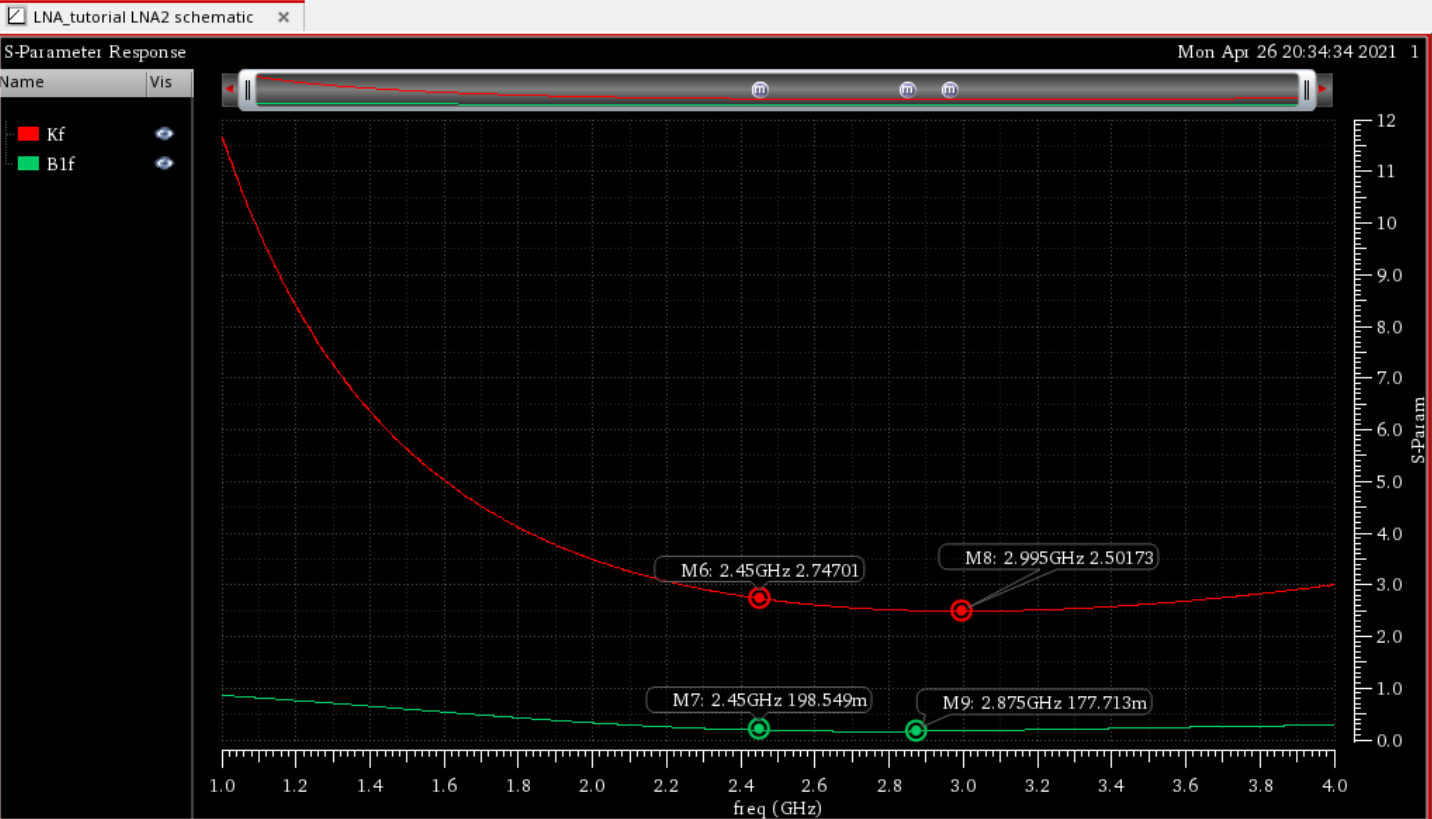
\includegraphics[scale=0.4]{5-3.png}
   \caption{Stability parameters plots}
\end{figure}


\begin{pexbox}{}
   \noindent \textbf{Is the LNA unconditionally stable?}
\end{pexbox}

   \noindent Yes, according to the conditions $K_f>1$ and $B_{1f}>0$.
 


\section{Evaluating Noise performance}
\begin{pexbox}{}
   \noindent \textbf{Capture the plots of NF obtained, including markers at $f_0 = 2.45$ GHz.}
\end{pexbox}
   
   \noindent I've obtained the Noise Figure, NF, from ADE - Results - Direct Plot - Noise Figure, without using the Direct Plot.
\begin{figure} [H] \centering
   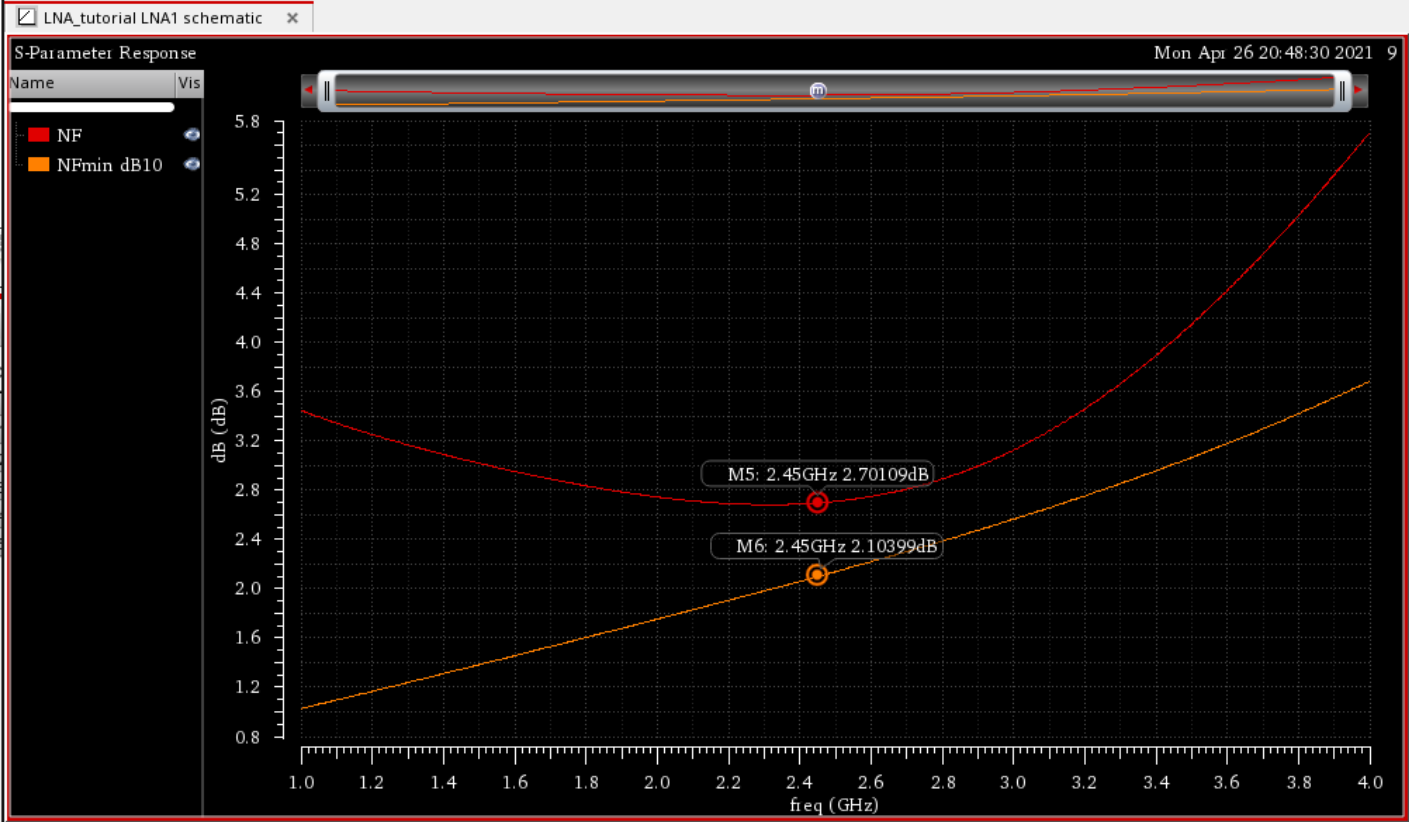
\includegraphics[scale=0.4]{6-1.png}
   \caption{NF plots}
\end{figure}


\begin{pexbox}{}
   \noindent \textbf{Is the NF close to the value theoretically expected?}
\end{pexbox}
   
   \noindent The theoretical value, with the professor's numbers, is
   \begin{equation}
      NF = 2.6 = 4.15 \text{ dB} \ .
   \end{equation}
   \noindent This doesn't fulfill the desired NF, $NF < 3$ dB, but in the pre-lab we were told we could fix this by increasing the current consumption to increase $f_T$. 
   
   \noindent However, after the simulation, the obtained NF is better than the theoretical one, and it fulfills $NF < 3$ dB.

\begin{pexbox}{}
   \noindent \textbf{Does the LNA fulfill the targeted NF specification?}
\end{pexbox}

   \noindent As commented, yes. As commented in the lab, this analysis tends to be optimistic, as it is done after linearizing the equations. If a large-signal analysis was performed, NF would tend to be worse (larger).




\begin{pexbox}{}
   \noindent \textbf{Capture the (upper part of the) Noise Summary window.}
\end{pexbox}

\begin{figure} [H] \centering
   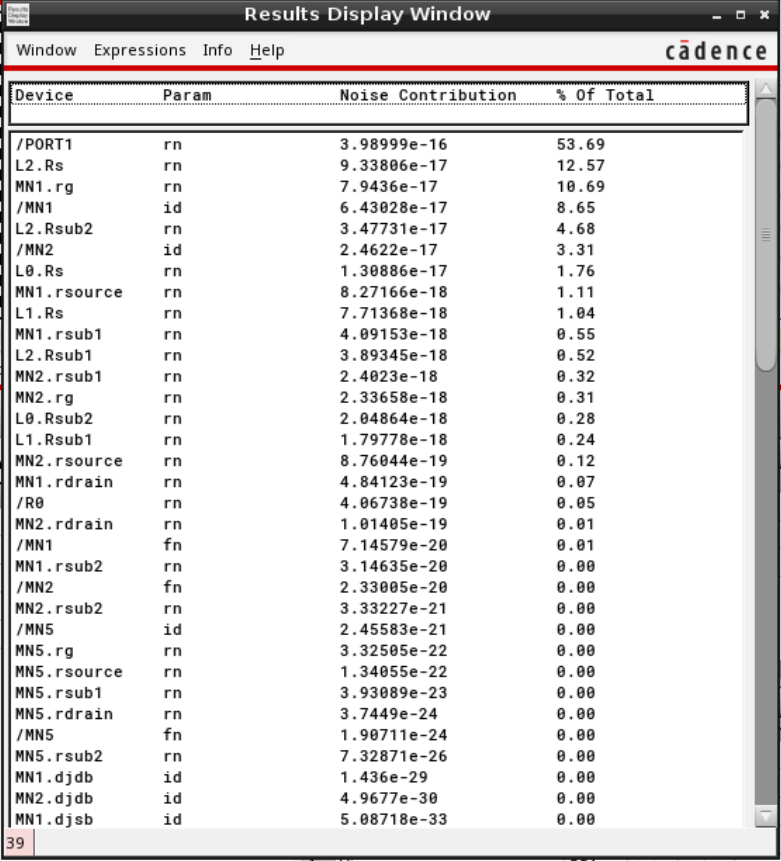
\includegraphics[scale=0.5]{6-2.png}
   \caption{Noise summary}
\end{figure}


\begin{pexbox}{}
   \noindent \textbf{Identify the noise sources that contribute more than 5\% to the total noise.}
\end{pexbox}

   \noindent As can be seen from the figure, only $4$ noise sources contribute more than $5$\% to the total noise. It's required to understand their origin.
   \begin{equation}
      \begin{split}
         /PORT1 &:  \text{Input voltage source 50 $\Omega$ equivalent resistance} \\
         L2.Rs &:  \text{Gate inductance series resistor} \\
         MN1.rg &:  \text{Input NMOS equivalent gate resistance} \\
         MN1 &:  \text{Input NMOS channel noise} \\
      \end{split} \ .
   \end{equation}

\begin{pexbox}{}
   \noindent \textbf{What does it mean that noise of PORT1 contributes more than 50\%?}
\end{pexbox}

   \noindent That the majority of the noise at the output comes from the input equivalent circuit, and thus that the LNA noise contribution is lower than the source one. The $NF=2.7$ dB is equal to $1.365$ in linear units. Recall
   \begin{equation}
      F = 1 + \frac{R_{Lg}}{R_s} + \frac{R_{Rg}}{R_s} + \frac{\gamma}{\alpha} g_m R_s \left(\frac{w_0}{w_T}\right)^2 \ .
   \end{equation}
   \noindent And we normally used
   \begin{equation}
      F_{min} = 1 + \frac{R_{Lg}}{R_s} + \frac{R_{Rg}}{R_s} + 2.4 \frac{\gamma}{\alpha} \frac{w_0}{w_T} \ .
   \end{equation}
   \noindent In our analysis, we neglected the NMOS equivalent gate resistance contribution. In the pre-lab, we had $R_{Lg} = 16 \ \Omega$. We calculated $f_T = 11.2$ GHz and we were given $\gamma = 2$, $\alpha = 0.8$. This lead us to $F = 2.6$. 

\begin{pexbox}{}
   \noindent \textbf{Is the contribution of the gate inductor $L_G$ larger of smaller than that calculated?}
\end{pexbox}

   \noindent Now, we have
   \begin{equation}
      \frac{R_{Lg}}{R_s} = \frac{L2.Rs}{/PORT1} = 0.234 \ .
   \end{equation}
   \noindent Before, with $R_{Lg} = 16 \ \Omega$, $\frac{R_{Lg}}{R_s} = 0.32$. So, the gate inductor contribution is lower, now.



\begin{pexbox}{}
   \noindent \textbf{Is the contribution of the channel thermal noise larger of smaller than that calculated?}
\end{pexbox}

   \noindent Now, we have
   \begin{equation}
       2.4 \frac{\gamma}{\alpha} \frac{w_0}{w_T} = \frac{MN1}{/PORT1} = 0.16 \ .
   \end{equation}
   \noindent While before this term was $\frac{\gamma}{\alpha} \frac{w_0}{w_T} = 1.267$. So, the simulation attributes less noise to the channel than the one we calculated. It helps that $w_T$ is greater than in the pre-lab calculations, as shown in a table before. The low channel termal noise is the main source of noise improvement.
   % segur?


% unitats del summary son V^2, canvia algo aixo???

\begin{pexbox}{}
   \noindent \textbf{Is the value of the gate resistance coherent with the contribution to the total output noise? Justify your answer}
\end{pexbox}

\noindent The gate resistance value I get is $R_g = 10.63 \ \Omega$.
\begin{figure} [H] \centering
   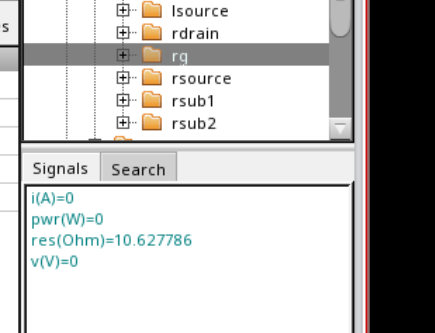
\includegraphics[scale=0.45]{6-rg.png}
   \caption{$R_g$ value at the CS transistor}
\end{figure}
\noindent So, it's contribution to the total noise should be $\frac{R_g}{R_s} = \frac{10.63}{50} = 0.2126$, normalized to the source noise (/PORT1). In the noise summary, the relation is $\frac{10.69}{53.69} = 0.199$. So, the value of the gate resistance is coherent with the contribution to the total output noise.


\begin{pexbox}{}
   \noindent \textbf{Optional: You can try to improve the NF by decreasing the gate resistance. We know this resistance can be reduced by layout, i.e. decreasing the finger size (and increasing the number of fingers, to preserve the total width).}
\end{pexbox}

\noindent I've decreased from $10$ to $5$ the stripe width, and instead of $N$ now I've set $2N$. A small decrease of noise results.
\begin{figure} [H] \centering
   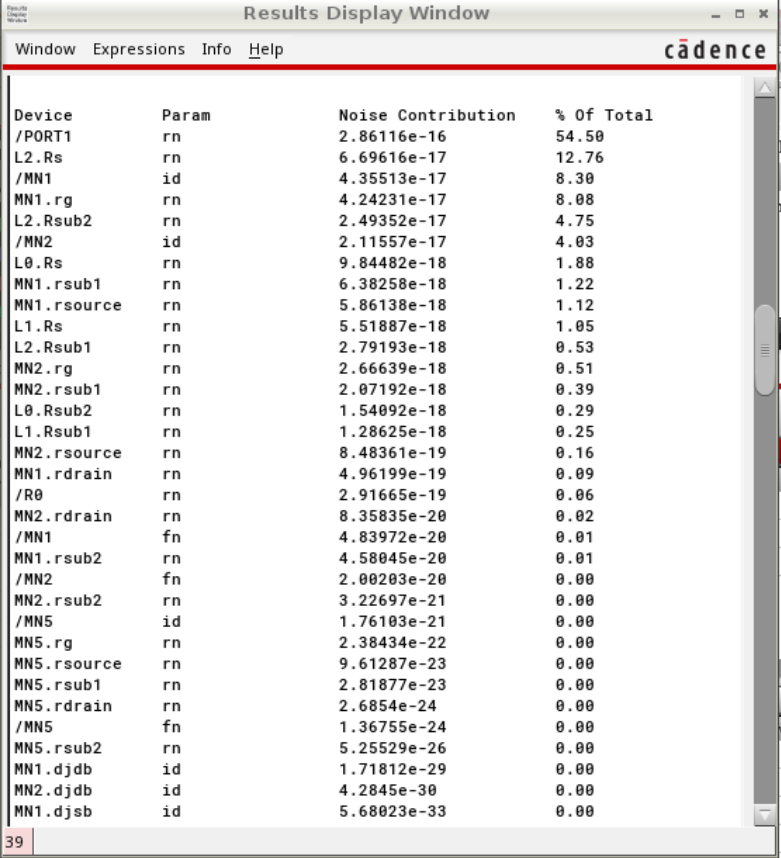
\includegraphics[scale=0.45]{6-2v2.png}
   \caption{Noise summary}
\end{figure}
\noindent Now the contribution from the gate resistance is the previous noise by a factor of $\approx 0.534$, so the improvement is noticeable. Still, in both cases the contribution is quite small overall, so there's not a huge impact on the total noise.





\section{Evaluating Linearity}

\begin{pexbox}{}
   \noindent \textbf{Capture the plot generated for the measurement of IP3.}
\end{pexbox}

\begin{figure} [H] \centering
   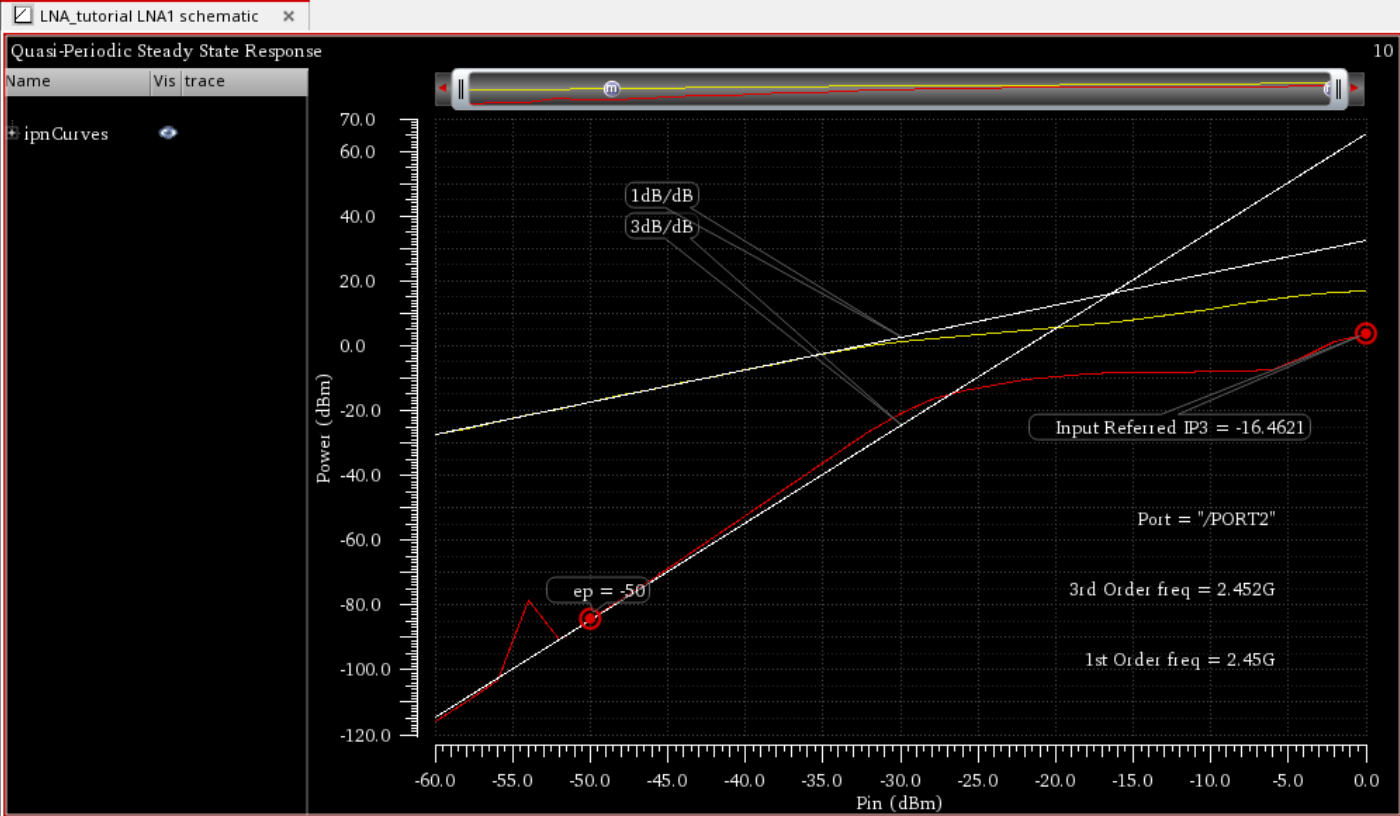
\includegraphics[scale=0.3]{7v0205.png}
   \caption{IP3 analysis}
\end{figure}


\begin{pexbox}{}
   \noindent \textbf{Which is the input-referred IP3 of your LNA?}
\end{pexbox}

   \noindent I get
   \begin{equation}
     % IIP3 = -2.36571 \text{ dBm} \ .
     IIP3 = -16.4621 \text{ dBm} \ .
   \end{equation}

\begin{pexbox}{}
   \noindent \textbf{Which is the OIP3?}
\end{pexbox}

   \noindent Taking the previous $A_v = 33$ dB, I would have
   \begin{equation}
      % OIP3 = 30.634 \text{ dBm} \ .
      OIP3 = 16.54 \text{ dBm} \ .
   \end{equation}
   \noindent This value can be, more or less, deduced on the previous plot, in the vertical axis.

\begin{pexbox}{}
   \noindent \textbf{Which other frequencies you could have selected for the fundamental tone and for the 3rd-order intermodulation product?}
\end{pexbox}

   \noindent The chosen frequencies, $f_1 = 2.45$ GHz and $f_2 = 2.451$ GHz result in third-order tones at $2.452$ GHz and $2.448$ GHz, and thus I've chosen $2.45$ GHz as the $1^{st}$ order harmonic, and $2.452$ GHz as the $3^{rd}$ order harmonic. I could have also chosen $2.451$ GHz as the $1^{st}$ order harmonic, and $2.449$ GHz as the $3^{rd}$ order harmonic, because the two input tones are of the same power, and the tone at $2.449$ GHz will be equal to the one at $2.451$ GHz. I've noticed that for this, the results were almost identical.







\begin{pexbox}{}
   \noindent \textbf{Capture the plot generated for the measurement of CP1dB.}
\end{pexbox}

\begin{figure} [H] \centering
   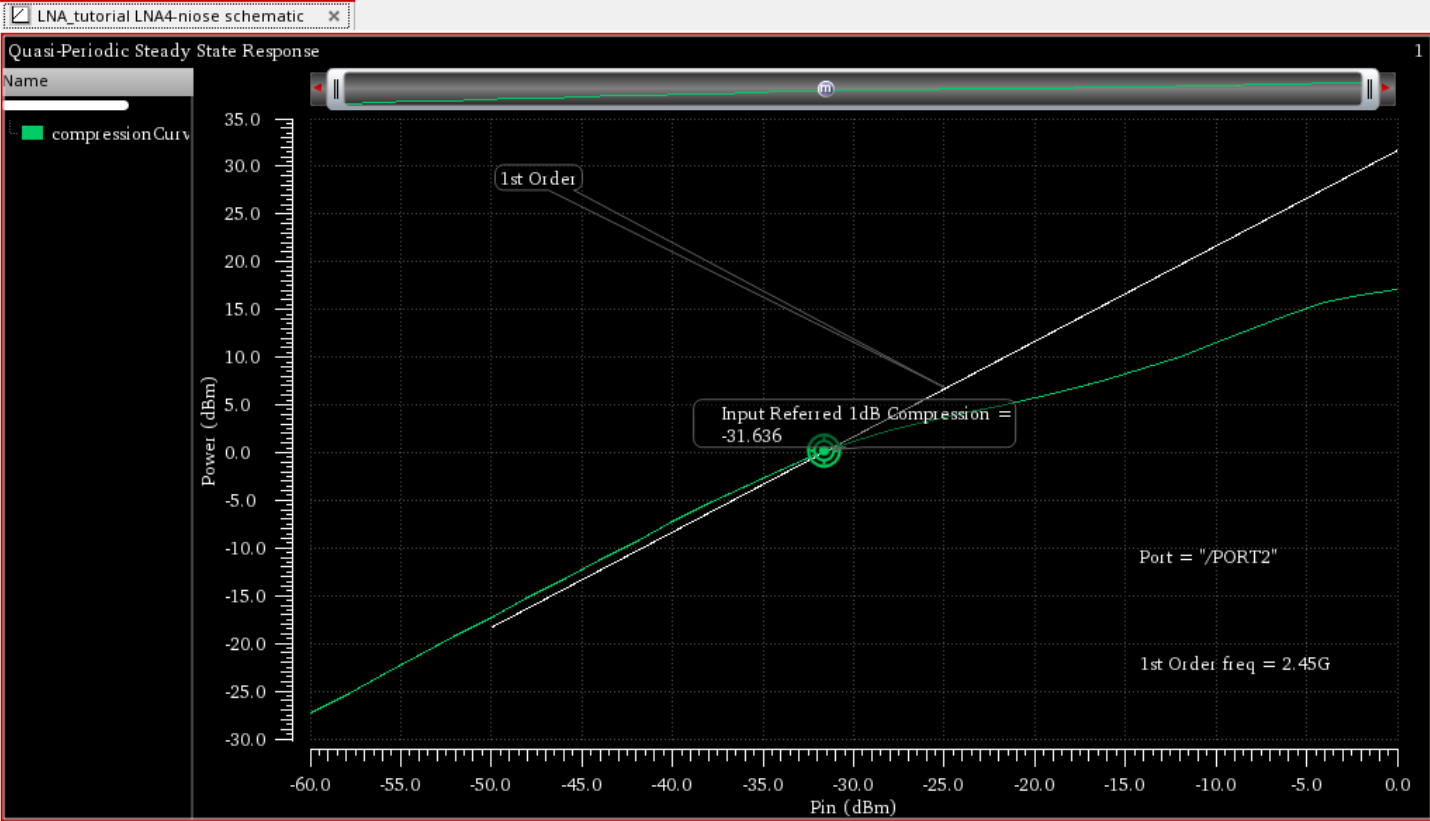
\includegraphics[scale=0.3]{7-comp-0205.png}
   \caption{Compression analysis}
\end{figure}


\begin{pexbox}{}
   \noindent \textbf{Which is the input-referred 1dB Compression point of your LNA?}
\end{pexbox}

   \noindent I get
   \begin{equation}
      P_{in,-1dB} = -31.636 \text{ dBm} \ .
   \end{equation}


\begin{pexbox}{}
   \noindent \textbf{Which is peak input amplitude that corresponds to this CP1dB?}
\end{pexbox}

\noindent By recalling that 
\begin{equation}
   P [dBm] = 10 \log\left(\frac{\frac{(V_{peak}/\sqrt{2})^2}{50}}{1 \text{ mW}}\right) \ ,
\end{equation}
\noindent I get
\begin{equation}
   V_{in,peak,-1dB} = 8.283 \text{ mV}_{peak} \ .
\end{equation}

\begin{pexbox}{}
   \noindent \textbf{Which is the output-referred 1dB Compression point of your LNA?}
\end{pexbox}
%
   \begin{equation}
      P_{out,-1dB} = 1.364 \text{ dBm} \ .
   \end{equation}


\begin{pexbox}{}
   \noindent \textbf{Which is peak output amplitude that corresponds to this CP1dB?}
\end{pexbox}

   \noindent A similar calculation to the one before is performed. I get
   \begin{equation}
      V_{out,peak,-1dB} = 0.370 \text{ V}_{peak} \ .
   \end{equation}









\begin{pexbox}{}
   \noindent \textbf{Optional: it is interesting that you repeat the 1dB compression point representation, but now selecting Power Gain as the output format representation. This provides an alternative interpretation of the 1dB compression point. At small input power, the gain is constant, and the 1dB compression point is the power at which the gain is reduced 1dB.}
\end{pexbox}

\begin{figure} [H] \centering
   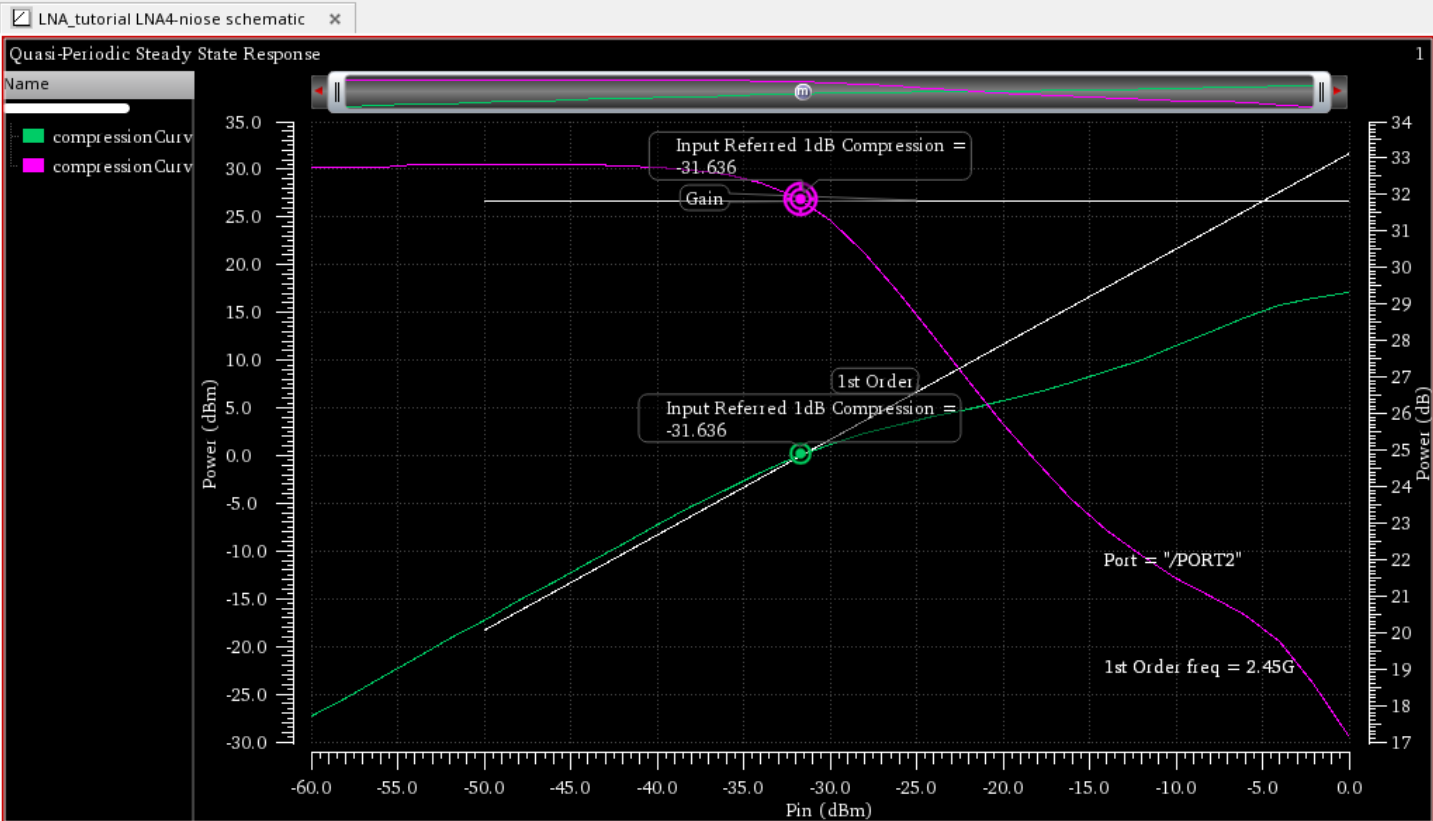
\includegraphics[scale=0.3]{7-compout-0205.png}
   \caption{Compression analysis}
\end{figure}


\noindent I have done it and the resulting plot is more or less as the statement says. For low input powers the response is more or less flat, and for high inputs compression starts taking place and the gain diminishes. The marked compression point is the same as before.




\section{Performance Summary}
\begin{pexbox}{}
   \noindent \textbf{Report the final performance results obtained, fulfilling the next table:}
\end{pexbox}

\noindent I've obtained different $S_{21}$ values during this lab. Some were obtained when there were mismatches, or when the buffer was deleted. We are told "LNA output voltage will drive the input of an on-chip mixer, thus LNA output impedance is not intended to be matched", so it makes more sense to take the first $S_{21}$ I obtained.
\begin{table}[H] \centering
   \begin{tabular}{ |l|r| } \hline
       Characteristic & Value \\ \hline \hline
       Central frequency $f_0$ & $2.45$ GHz \\ \hline % $\approx 2.4$ GHz, designed for 
       S21 (dB) & $32.9953$  \\ \hline % amb buffer, sino 8.4 dB...
       NF & $2.70109$ dB \\ \hline
       IIP3 (dBm) & $-16.4621$ \\ \hline
       Input - CP 1dB (dBm) & $-31.636$ \\ \hline
       S11 (dB) &  $-9.80$ \\ \hline
       Reverse Isolation, S12 (dB) & $-37.435$ \\ \hline
       VDD & $3.3$ V \\ \hline
       IDC (mA) & $2.629$ \\ \hline
       Power Dissipation (mW) & $8.6757$ \\ \hline
       Technology Process & C35B4M3, $0.35 \ \mu$m \\ \hline
   \end{tabular}
   \caption{Final performance results}
\end{table}


% \begin{table}[H] \centering
   % \begin{tabular}{ |l|r| } \hline
       % Characteristic & Value \\ \hline \hline
       % Central frequency $f_0$ & $2.45$ GHz \\ \hline % $\approx 2.4$ GHz, designed for 
       % S21 (dB) & $32.9953$  \\ \hline % amb buffer, sino 8.4 dB...
       % NF & $2.70109$ dB \\ \hline
       % IIP3 (dBm) & $-2.36571$ \\ \hline
       % Input - CP 1dB (dBm) & $1.13416$ \\ \hline
       % S11 (dB) &  $-9.80$ \\ \hline
       % Reverse Isolation, S12 (dB) & $-37.435$ \\ \hline
       % VDD & $3.3$ V \\ \hline
       % IDC (mA) & $2.629$ \\ \hline
       % Power Dissipation (mW) & $8.6757$ \\ \hline
       % Technology Process & C35B4M3, $0.35 \ \mu$m \\ \hline
   % \end{tabular}
   % \caption{Final performance results}
% \end{table}
% quan trec el buffer baixa molt el S21, suposo que es desperar, pero tant petit...

\begin{pexbox}{}
   \noindent \textbf{Optional: You may want to compare the LNA performance you obtained against the performance of LNA designed by international research groups, published in research journals of congresses. A fair comparison would restrict to LNAs designed in similar technology nodes, similar central frequencies, single-ended topologies. We propose eg. the following works:}
\end{pexbox}

\begin{table}[H] \centering
   \begin{tabular}{ |l|r|r|r| } \hline
       Characteristic & LNA lab & Song & Shaeffer \\ \hline \hline
       Central frequency $f_0$ & $2.45$ GHz & $2.1$ GHz & $1.5$ GHz \\ \hline % $\approx 2.4$ GHz, designed for 
       S21 (dB) & $32.9953$ & $16.4$ & $22$  \\ \hline % amb buffer, sino 8.4 dB...
       NF & $2.70109$ dB & $2.77$ dB & $3.5$ dB \\ \hline
       IIP3 (dBm) & $-16.4621$ & $7.45$ & $-9.3$ \\ \hline
       Input - CP 1dB (dBm) & $-31.636$ & - & $-22$  \\ \hline
       S11 (dB) &  $-9.80$ & $-19.7$ & $1.385$ (?) \\ \hline
       Reverse Isolation, S12 (dB) & $-37.435$ & $-33.4$ & $-42.451$  \\ \hline
       VDD & $3.3$ V & $1.8$ V & $1.5$ V \\ \hline
       IDC (mA) & $2.629$ & $13.88$ & $20$  \\ \hline
       Power Dissipation (mW) & $8.6757$ & $25$ & $30$  \\ \hline
       Technology Process & C35B4M3, $0.35 \ \mu$m & $0.25 \ \mu$m & $0.6 \ \mu$m  \\ \hline
   \end{tabular}
   \caption{Comparison table}
\end{table}
% quan trec el buffer baixa molt el S21, suposo que es desperar, pero tant petit... a veure que respon

% \begin{table}[H] \centering
   % \begin{tabular}{ |l|r|r|r| } \hline
       % Characteristic & LNA lab & Song & Shaeffer \\ \hline \hline
       % Central frequency $f_0$ & $2.45$ GHz & $2.1$ GHz & $1.5$ GHz \\ \hline % $\approx 2.4$ GHz, designed for 
       % S21 (dB) & $32.9953$ & $16.4$ & $22$  \\ \hline % amb buffer, sino 8.4 dB...
       % NF & $2.70109$ dB & $2.77$ dB & $3.5$ dB \\ \hline
       % IIP3 (dBm) & $-2.36571$ & $7.45$ & $-9.3$ \\ \hline
       % Input - CP 1dB (dBm) & $1.13416$ & - & $-22$  \\ \hline
       % S11 (dB) &  $-9.80$ & $-19.7$ & $1.385$ (?) \\ \hline
       % Reverse Isolation, S12 (dB) & $-37.435$ & $-33.4$ & $-42.451$  \\ \hline
       % VDD & $3.3$ V & $1.8$ V & $1.5$ V \\ \hline
       % IDC (mA) & $2.629$ & $13.88$ & $20$  \\ \hline
       % Power Dissipation (mW) & $8.6757$ & $25$ & $30$  \\ \hline
       % Technology Process & C35B4M3, $0.35 \ \mu$m & $0.25 \ \mu$m & $0.6 \ \mu$m  \\ \hline
   % \end{tabular}
   % \caption{Comparison table}
% \end{table}
% quan trec el buffer baixa molt el S21, suposo que es desperar, pero tant petit... a veure que respon







\begin{pexbox}{}
   \noindent \textbf{Optional: Performance comparison to other circuits may be difficult if they operate at different central frequencies. Also, different performance can be traded-off, thus one metric (eg gain) can be better than your work, while other (eg. linearity) can be worse. To ease comparison, Figures of Merit (FoM) have bee defined, that ease comparison.}

   \noindent \textbf{We propose you compare your LNA against the designed published in other works, in
   terms of the following FoM:}
   \begin{equation}
      FoM_1 (GHz) = \frac{G_p(lin) \cdot f_0 (GHz) \cdot IIP3 (mW) }{ \left(F(lin) - 1\right) \cdot Power (mW) } \ .
   \end{equation}
\end{pexbox}

\noindent I guess $G_p (lin)$ is the $S_{21}$ in linear units. Some intermediate calculations:
\begin{equation}
   \begin{split}
   S_{21} \text{ linear} &= 44.61, \ 6.6069, \ 12.589 \\ 
   \text{NF linear} &= 1.86, \ 1.89, \ 2.239 \\ 
   IIP3 \text{ [mW]} &= 0.02258, \ 5.559, \ 0.1175 \\ 
   \end{split}
\end{equation}
% S21 linear: 44.61, 6.6069, 12.589. Si pillo 8.4 dB, 2.63
% NF linear: 1.86, 1.89, 2.239
% IIP3 en mW: 0.58, 5.559, 0.1175. Now, 0.02258
\noindent I get
\begin{table}[H] \centering
   \begin{tabular}{ |l|r|r|r| } \hline
       Characteristic & LNA lab & Song & Shaeffer \\ \hline \hline
       $FoM_1$ (GHz) & $0.3307$ GHz & $3.466$ GHz & $0.05969$ GHz \\ \hline % agafant 8.4dB, 0.5 GHz, el meu
   \end{tabular}
   \caption{Comparison table}
\end{table}
% quan trec el buffer baixa molt el S21, suposo que es desperar, pero tant petit... a veure que respon
 
\noindent To my surprise, I've been able to get a better figure of merit than the one that from Shaeffer results. One reason may be that Shaeffer paper is quite old, and that I may be using a better technology. The other is that this figure of merit considers a lot of variables, and that the comparison may not be totally fair.
























% \chapter{LNA PreLab}


% \begin{pexbox}
   % \noindent \textbf{1.‐ As a first step, you wil try to obtain the targeted performance with the  cheapest technology option, C35B4C3. Find the required gm according to the Gain specification.  Then estimate the current consumption, input matching and NF achieved. Do not redo your design for those targets, even if they are not fulfilled.}

   % \noindent \textbf{Report the following information for your design, and expected performance.}
% \end{pexbox}


% \noindent The circuit to implement will be:
% \begin{figure}[H]
   % \centering
   % \begin{circuitikz}[>=latex'][american]
   % \tikzstyle{block} = [draw, rectangle, minimum height=1cm, minimum width=2cm]
   % \ctikzset{tripoles/mos style/arrows}
   % \ctikzset{tripoles/pmos style/nocircle}
   % \draw (4.5,1.5) node[nmos](Q1){Q1};\draw (Q1.D) to[short] (4.5,2.5);
   % \draw (Q1.S) to[short] (4.5,0.5);
   % \draw (Q1.G) to[short] (3.5,1.5);
   % \draw (4.5,-1.0) node[nmos](Q2){Q2};\draw (Q2.D) to[short] (4.5,-0.0);
   % \draw (Q2.S) to[short] (4.5,-2.0);
   % \draw (Q2.G) to[short] (3.5,-1.0);
   % \draw (4.5,-2.0) to[L,l=$L_S$] (4.5,-3.5);
   % \draw (3.5,-1.0) to[L,l=$L_G$] (1.5,-1.0);
   % \draw (4.5,2.5) to[L,l=$L_D$] (4.5,4.0);
   % \draw (7.0,2.5) to[C,l=$C_L$] (7.0,0.5);
   % \draw (-1.0,-1.0) node[nmos](Q4){Q4};\draw (Q4.D) to[short] (-1.0,-0.0);
   % \draw (Q4.S) to[short] (-1.0,-2.0);
   % \draw (Q4.G) to[short] (-2.0,-1.0);
   % \draw (1.5,-1.0) to[R,l=$R$] (0.0,-1.0);
   % \draw (-1.0,4.0) to[isource,l=$I_{ref}$] (-1.0,-0.0);
   % \draw (7.0,0.5) node[ground]{};
   % \draw (4.5,-3.5) node[ground]{};
   % \draw (1.5,-1.0) to[C,l=$C_{dec}$] (1.5,-3.0);
   % \draw (1.5,-3.0) to[R,l=$R_S$] (-0.5,-3.0);
   % \draw (-1.0,-2.0) node[ground]{};
   % \draw (-1.5,-1.0) to[short] (0.0,-1.0);
   % \draw (-1.0,-0.0) to[short] (0.0,-0.0);
   % \draw (0.0,-0.0) to[short] (0.0,-1.0);
   % \draw (-1.0,4.0) to[short] (4.5,4.0);
   % \draw (7.0,2.5) to[short] (4.5,2.5);
   % \draw (4.5,0.5) to[short] (4.5,-0.0);
   % \draw (3.5,1.5) to[short] (3.5,4.0);
   % \draw (-1.0,-3.3) node[] {$v_{in}$};
   % \draw (2.0,4.0) node[vcc]{$V_{DD}$};
   % \end{circuitikz}
   % \caption{LNA amplifier}
   % \end{figure}


% \noindent First of all, it's needed to find the optimum transistor width, $W_{opt}$. From course slides, it's a good assumption to take $Q_{s,opt}=4.5$ in the following equation:
% \begin{equation}
   % W_{opt} = \frac{3}{2} \frac{1}{w_0 L C_{ox} R_s Q_{s,opt}} \ .
% \end{equation}
% \noindent Where $w_0 = 2 \pi f_0 = 2 \pi 2.45 \cdot 10^{9}$, $L = 0.35 \ \mu$m, $C_{ox} = 4.5 \text{ fF/}\mu\text{m}^2$ and $R_s = 50 \ \Omega$. With this,
% \begin{equation}
   % W_{opt} = 274.968 \ \mu\text{m} \approx 270 \ \mu\text{m} \ .
% \end{equation}
% \noindent With this width value $C_{GS}$, $C_{GD}$ and $C_{BD}$ can be calculated.
% \begin{equation}
   % \begin{split}
      % C_{GS} &= \frac{2}{3} W L C_{ox}  + C_{ov} = 310.5 \text{ fF} \\
      % C_{GD} &= W C_{ov} = 27 \text{ fF} \\
      % C_{DB} &= W C_{db} = 94.5 \text{ fF} \\
   % \end{split} \ .
% \end{equation}
% \noindent Where $C_{db} = 0.35 \text{ fF/}\mu\text{m}$ and $C_{ov} = 0.1 \text{ fF/}\mu\text{m}$.

% \noindent With this, the output capacitance plus the load capacitance is known.
% \begin{equation}
   % C_{OUT} = C_L + C_{GD} + C_{DB} = 621.5 \text{ fF} \ .
% \end{equation}
% \noindent This output capacitance must ressonate with $L_D$. So,
% \begin{equation}
   % L_D w_0 = \frac{1}{C_{OUT} w_0} \ .
% \end{equation}
% \noindent This leads to
% \begin{equation}
   % \boxed{
      % L_D = 6.79 \text{ nH} \rightarrow L_D = 5.52 \text{ nH} , \ Q=3.4
   % }
% \end{equation}
% \noindent The inductance value has been approximated to the closest one in the library. We know
% \begin{equation}
   % R_{D,s} = \frac{w L_{D,s}}{Q} \ .
% \end{equation}
% \noindent Where $w = w_0$, and $L_{D,s} \approx L_D \approx 5.62$ nH, as I take the inductance value at $2.4$ GHz, which is very close to $f_0$. Then,
% \begin{equation}
   % R_{D,s} = 25.445 \ \Omega \ .
% \end{equation}
% \noindent It is known that the equivalent paralel resistance is 
% \begin{equation}
   % R_{D,p} = R_{D,s} \left(1 + Q^2 \right) = 319.6 \ \Omega \ .
% \end{equation}
% \noindent As $A_v = G_m R_{D,p}$, we have that $G_m = 0.0989$ A/V. Establishing
% \begin{equation}
   % G_m = \frac{\frac{g_m}{C_{GD} + C_{GS}}}{w_0 \left(R_s + Z_{in} \right)} \ ,
% \end{equation}
% \noindent and that ideally $Z_{in} = R_s$, 
% \begin{equation}
   % g_m = 51.38 \text{ mA/V} \ .
% \end{equation}
% \noindent As $g_m = \sqrt{2 k' \frac{W}{L} I_D}$,
% \begin{equation}
   % I_D = 10.065 \text{ mA} \ .
% \end{equation}
% \noindent Which is way higher than the maximum current.

% \noindent Now, we should be able to match the source impedance $R_s = 50 \ \Omega$ to the input impedance of the LNA, $Z_{in}$.
% \begin{equation}
   % Z_{in} = \frac{1}{j w C_{GS}} + jw \left(L_S + L_G \right) + L_S \frac{g_m}{C_{GS} + C_{GD}} \ .
% \end{equation}
% \noindent So,
% \begin{equation}
   % R_s = 50 \ \Omega = L_S \frac{g_m}{C_{GS} + C_{GD}} \ .
% \end{equation}
% \noindent Leading to
% \begin{equation}
   % \boxed{
      % L_S = 0.328 \text{ nH} \rightarrow L_S = 1.37 \text{ nH}, \ Q = 6.1
   % }
% \end{equation}
% \noindent Finally, from the $Z_{in}$ expression we want the imaginary part to be $0 \ \Omega$. So,
% \begin{equation}
   % L_S + L_G = \frac{1}{w_0^2 C_{GS}} = 13.5908 \text{ nH} \ .
% \end{equation}
% \noindent $L_S$ is already known, thus
% \begin{equation}
   % \boxed{
      % L_G = 12.22 \text{ nH} \rightarrow 9.15 \text{ nH} , \ Q=3.3
   % }
% \end{equation}
% \noindent Performing a similar calculation as before for the equivalent series resistance, gets me
% \begin{equation}
   % R_{G,s} = 46.55 \ \Omega \ .
% \end{equation}
% \noindent The real part of $Z_{in}$ is recalculated.
% \begin{equation}
   % Re(Z_{in}) = L_S \frac{g_m}{C_{GS} + C_{GD}} = 208.84 \ \Omega \ .
% \end{equation}
% \noindent The actual $G_v$ is
% \begin{equation}
   % G_v = \frac{w_T}{w_0 \left(R_s + Re(Z_{in}) \right)} = 38.208 \text{ mA/V} \ .
% \end{equation}




% \noindent Finally, the noise figure can be calculated.
% \begin{equation}
   % F = 1 + \frac{R_{Lg}}{R_s} + \frac{\gamma}{\alpha} g_m R_S \left(\frac{w_0}{w_T}\right) \ .
% \end{equation}
% \noindent The transistion angular frequency was not explicitely calculated, but it is now.
% \begin{equation}
   % w_T = \frac{g_m}{C_{GS} + C_{GD}} = 1.5224 \cdot 10^{11} \text{ rad/s} \ .
% \end{equation}
% \noindent With this,
% \begin{equation}
   % F = 1 + 0.931 + 0.25626 = 1.996668 \ .
% \end{equation}
% \noindent Thus,
% \begin{equation}
   % NF = 10 \log(F) = 3.399 \text{ dB} \ .
% \end{equation}


% \noindent All the results are tabulated in the following table.


% \begin{table}[H] \centering
   % \begin{tabular}{ |l|l| } \hline
       % Characteristic & Value \\ \hline \hline
       % $L_D$ & $5.52$ nH \\ \hline
       % $Q \ (L_D)$ & $3.4$ \\ \hline
       % $L_S$ & $1.37$ nH  \\ \hline
       % $Q \ (L_S)$ & $6.1$  \\ \hline
       % $L_G$ & $9.15$ nH \\ \hline
       % $Q \ (L_G)$ & $3.3$ \\ \hline
       % Width$_{total}$ & $270 \ \mu$m \\ \hline
       % $C_{gg}$ & $337.5$ fF \\ \hline
       % $g_m$ & $51.38$ mA/V \\ \hline
       % $f_T$ & $1.52237 \cdot 10^{11} / (2 \pi) = 24.23$ GHz \\ \hline
       % $I_{DC}$ & $10.065$ mA \\ \hline
       % $Re(Z_{in})$ & $208.84 \ \Omega$ \\ \hline
       % $G_v$ & $38.208$ mA/V \\ \hline
       % $NF$ & $3.399$ dB \\ \hline
   % \end{tabular}
   % \caption{Results table}
% \end{table}




% \begin{pexbox}
   % \noindent \textbf{2.‐ In view of the results with the C35B4C3 process, next step is to try with a more expensive process option, the C35B4M3. Repeat the former design steps, now taking the inductors of the C35B4M3 library. Find the required gm according to the Gain specification. Then estimate the current consumption, input matching and NF achieved. Do not redo your design for those targets, even if they are not fulfilled.}

   % \noindent \textbf{Report the following information for your design, and expected performance:}
% \end{pexbox}

% \noindent The previous procedure is exactly replicated here, but now the expensive library, C35B4M3, is used for the inductors.


% %%
% \noindent First of all, it's needed to find the optimum transistor width, $W_{opt}$. From course slides, it's a good assumption to take $Q_{s,opt}=4.5$. The optimum width is exactly the same as before.
% \begin{equation}
   % W_{opt} = 274.968 \ \mu\text{m} \approx 270 \ \mu\text{m} \ .
% \end{equation}
% \noindent With this width value $C_{GS}$, $C_{GD}$ and $C_{BD}$ can be calculated, exactly as before.
% \begin{equation}
   % \begin{split}
      % C_{GS} &= \frac{2}{3} W L C_{ox}  + C_{ov} = 310.5 \text{ fF} \\
      % C_{GD} &= W C_{ov} = 27 \text{ fF} \\
      % C_{DB} &= W C_{db} = 94.5 \text{ fF} \\
   % \end{split} \ .
% \end{equation}
% \noindent Where $C_{db} = 0.35 \text{ fF/}\mu\text{m}$ and $C_{ov} = 0.1 \text{ fF/}\mu\text{m}$.

% \noindent With this, the output capacitance plus the load capacitance is known.
% \begin{equation}
   % C_{OUT} = C_L + C_{GD} + C_{DB} = 621.5 \text{ fF} \ .
% \end{equation}
% \noindent This output capacitance must ressonate with $L_D$. So,
% \begin{equation}
   % L_D w_0 = \frac{1}{C_{OUT} w_0} \ .
% \end{equation}
% \noindent Here, there's the first difference with respect to the other libary. Now,
% \begin{equation}
   % \boxed{
      % L_D = 6.79 \text{ nH} \rightarrow L_D = 6.00 \text{ nH} , \ Q=6.8
   % }
% \end{equation}
% \noindent The inductance value has been approximated to the closest one in the library. We know
% \begin{equation}
   % R_{D,s} = \frac{w L_{D,s}}{Q} \ .
% \end{equation}
% \noindent Where $w = w_0$, and $L_{D,s} \approx L_D \approx 6.59$ nH, as I take the inductance value at $2.4$ GHz, which is very close to $f_0$. Then,
% \begin{equation}
   % R_{D,s} = 14.92 \ \Omega \ .
% \end{equation}
% \noindent It is known that the equivalent paralel resistance is 
% \begin{equation}
   % R_{D,p} = R_{D,s} \left(1 + Q^2 \right) = 704.75 \ \Omega \ .
% \end{equation}
% \noindent As $A_v = G_m R_{D,p}$, we have that $G_m = 0.0989$ A/V. Establishing
% \begin{equation}
   % G_m = \frac{\frac{g_m}{C_{GD} + C_{GS}}}{w_0 \left(R_s + Z_{in} \right)} \ ,
% \end{equation}
% \noindent and that ideally $Z_{in} = R_s$, 
% \begin{equation}
   % g_m = 21.45 \text{ mA/V} \ .
% \end{equation}
% \noindent As $g_m = \sqrt{2 k' \frac{W}{L} I_D}$,
% \begin{equation}
   % I_D = 1.757 \text{ mA} \ .
% \end{equation}
% \noindent A current mirror of 1:10 ratio will consume less than $2.5$ mA, so all good for now. 

% \noindent Now, we should be able to match the source impedance $R_s = 50 \ \Omega$ to the input impedance of the LNA, $Z_{in}$.
% \begin{equation}
   % Z_{in} = \frac{1}{j w C_{GS}} + jw \left(L_S + L_G \right) + L_S \frac{g_m}{C_{GS} + C_{GD}} \ .
% \end{equation}
% \noindent So,
% \begin{equation}
   % R_s = 50 \ \Omega = L_S \frac{g_m}{C_{GS} + C_{GD}} \ .
% \end{equation}
% \noindent Leading to
% \begin{equation}
   % \boxed{
      % L_S = 0.716 \text{ nH} \rightarrow L_S = 1.07 \text{ nH}, \ Q = 8.7
   % }
% \end{equation}
% \noindent Finally, from the $Z_{in}$ expression we want the imaginary part to be $0 \ \Omega$. So,
% \begin{equation}
   % L_S + L_G = \frac{1}{w_0^2 C_{GS}} = 13.5908 \text{ nH} \ .
% \end{equation}
% \noindent $L_S$ is already known, thus
% \begin{equation}
   % \boxed{
      % L_G = 12.52 \text{ nH} \rightarrow 10.02 \text{ nH} , \ Q=6.8
   % }
% \end{equation}
% \noindent Performing a similar calculation as before for the equivalent series resistance, gets me
% \begin{equation}
   % R_{G,s} = 27.355 \ \Omega \ .
% \end{equation}
% %
% \noindent The real part of $Z_{in}$ is recalculated,
% \begin{equation}
   % Re(Z_{in}) = L_S \frac{g_m}{C_{GS} + C_{GD}} = 73.324 \ \Omega \ .
% \end{equation}
% \noindent The actual $G_v$ is
% \begin{equation}
   % G_v = \frac{w_T}{w_0 \left(R_s + Re(Z_{in}) \right)} = 36.386 \text{ mA/V} \ .
% \end{equation}

% \noindent Finally, the noise figure can be calculated.
% \begin{equation}
   % F = 1 + \frac{R_{Lg}}{R_s} + \frac{\gamma}{\alpha} g_m R_S \left(\frac{w_0}{w_T}\right) \ .
% \end{equation}
% \noindent The transistion angular frequency was not explicitely calculated, but it is now.
% \begin{equation}
   % w_T = \frac{g_m}{C_{GS} + C_{GD}} = 1.5224 \cdot 10^{11} \text{ rad/s} \ .
% \end{equation}
% \noindent With this,
% \begin{equation}
   % F = 1 + 0.931 + 0.25626 = 1.996668 \ .
% \end{equation}
% \noindent Thus,
% \begin{equation}
   % NF = 10 \log(F) = 2.561 \text{ dB} \ .
% \end{equation}


% \noindent All the results are tabulated in the following table.
% %%


% \begin{table}[H] \centering
   % \begin{tabular}{ |l|r| } \hline
       % Characteristic & Value \\ \hline \hline
       % $L_D$ & $6.00$ nH \\ \hline
       % $Q \ (L_D)$ & $6.8$ \\ \hline
       % $L_S$ & $1.07$ nH  \\ \hline
       % $Q \ (L_S)$ & $8.7$  \\ \hline
       % $L_G$ & $10.02$ nH \\ \hline
       % $Q \ (L_G)$ & $6.8$ \\ \hline
       % Width$_{total}$ & $270 \ \mu$m \\ \hline
       % $C_{gg}$ & $337.5$ fF \\ \hline
       % $g_m$ & $21.45$ mA/V \\ \hline
       % $f_T$ & $6.356 \cdot 10^{10} / (2 \pi) = 10.012$ GHz \\ \hline
       % $I_{DC}$ & $1.757$ mA \\ \hline
       % $Re(Z_{in})$ & $73.324 \ \Omega$ \\ \hline
       % $G_v$ & $36.386$ mA/V \\ \hline
       % $NF$ & $2.561$ dB \\ \hline
   % \end{tabular}
   % \caption{Results table}
% \end{table}








% \begin{pexbox}
   % \noindent \textbf{3.‐ The DC current calculated before will be obtained with a current mirror with a 1:10 ratio, with the reference current produced by an ideal current source. Calculate the expected value of the reference current $I_{ref}$, to produce the targeted DC current, accounting for the error produced by the $V_{DS}$ dependence (channel‐length modulation). You can assume in your calculations an approximate $V_{OD} = 200$ mV, $V_G$ of the cascode transistor connected to $V_{DD}$, and neglect the body effect on $V_T$. Once you have calculated $I_{ref}$, you can calculate the expected actual $V_{OD}$.}
% \end{pexbox}

% \noindent Here, I opt to assume $V_{OD} = 200$ mV for the cascode transistor, so in the DC analysis the CS transistor will see $V_{DS} = 2.6$ V, because $V_T = 0.5$ V. Then, the CS overdrive voltage is calculated.
% \begin{equation}
   % I_{DQ} = 1.757 \text{ mA} = \frac{1}{2} k' \frac{W}{L} V_{OD}^2 \left(1 + \lambda V_{DS} \right) \ .
% \end{equation}
% \noindent This leads to 
% \begin{equation}
   % V_{OD} = 0.1388 \text{ V} \ .
% \end{equation}
% \noindent Thus, the voltage in the left transistor gate and drain, which is biased with $I_{ref}$, will be $0.1388 + V_T = 0.6388$ V. Then, $I_{ref}$ results.
% \begin{equation}
   % I_{ref} = \frac{1}{2} k' \left(\frac{W/L}{10}\right) V_{OD}^2 \left(1 + \lambda \left(V_{OD} + V_T \right)\right) \ .
% \end{equation}
% \noindent Recall we were told to use a 1:10 current mirror.
% \begin{equation}
   % \boxed{
      % I_{ref} = 138.43 \ \mu\text{A}
   % }
% \end{equation}



% \noindent Another option would have been to establish:
% \begin{equation}
   % \begin{split}
      % 1.757 \text{ mA} &= K V_{OD}^2 \left(1 + 2.6 \lambda \right) \\
      % I_{ref}  &= \frac{K}{10} V_{OD}^2 \left(1 + 0.7 \lambda \right) \\
   % \end{split} \ .
% \end{equation}
% \noindent This leads to $I_{ref} = 139.68 \ \mu$A, very close to the previous value. Notice it has not been necessary to calculate $V_{OD}$. 
 
